\chapter{Results}
In this chapter the results produced by the application of the different trading strategies are discussed, but first of all final instructions on the setup of the system are given. Since the simulation is far from being perfect, the analysis of the data will mostly be qualitative.
\section{Final Setup}
After the previously performed trading analysis in chapter \ref{chap:tradingDynamics} the configuration from scenario has been used in all further studies. The corresponding ini files can be found in the appendix in \ref{chap:iniContainment}. They resemble the description given in chapter \ref{chap:testedStrategiesDesc}.  
In order to keep the runtime reasonable for this thesis and testing, farms with a smaller size than 20 cows have been excluded from the simulation. The argument for this is that small farms can not build a sustainable business and are rather run by families, which want to make some money besides their daytime jobs. They will most likely not buy and sell cows all the time and therefore not play a big role in the spreading of BVD on the network. This assumption has not been proven by now. \citep{steinbach16} provided a categorisation of nodes based on their trading behavior as markets, traders, self-sustaining premises, fattening and breeding farms. This method could be refined to build a more realistic model of the market in the future. 
Applying this idea removes $15272\cows$ ($4.46\,\%$) in $5544\,\text{farms}$ ($82.16\,\%$).
Since the behavior of the different farms has not been studied and implemented in this simulation fully and because the system size in terms of farms is much smaller than the actual network size of all of Thuringia, the implementation of a more refined and realistic market behavior has been postponed. 
The data given in chapter \ref {chap:rlDataRegulationGermany} has been used to set up the system. This was done by randomly choosing $2\,\%$ of the farms to be set up with the shares of the different compartments of previously with PIs contaminated farms. The other $98\,\%$ of the farms were set up with the shares of all compartments corresponding to now previous contamination by PIs. With all these measures taken multiple simulations where run. The global prevalence strongly depends on the farms chosen to be infected in the beginning. If smaller farms are contaminated in the beginning, the disease will need much longer to spread or even die out, since far less animals are infected and the in- and out-degree of these small farms are relatively small, which leads to a smaller infection rate for all other nodes. With the aim of limiting the amount of scenarios to be discussed, one scenario which exposed a prevalence close to the big single farm with approximately $40000\cows$ from section \ref{chap:diseaseDynamicsDesc} has been chosen. It exhibited the highest global prevalence after $20\days$. The seed from this run is used in all runs for the different strategies, to make sure that the transients for the system for all strategies look exactly the same. By setting the seed of the random number generator, two streams of random numbers produced by this random number generator will be exactly the same. This is used to have the same events happen during the transient phase for all strategies, leading to results, which can be compared. The containment strategies in each scenario are turned on on a global scale after $10000\days$. 
The cow well farm still introduces pregnant cows, $2\,\%$ of which are PIs, into the system, which exceeds the most pessimistic guess of $1.5\,\%$ by \citep{personalCom}, which was based on import data from HIT and EuroStat.  
\section{Strategy I - No Strategy}
This first run corresponds to the control group in clinical tests of medication. As can be seen in figure \ref{fig:cont1Behav}, the simulation reaches a stable state with some smaller oscillations between $5000\text{ and } 10000\days$. The total number of animals stabilizes slightly beneath its initial value of $326439\cows$ at approximately $316000\cows$. The numbers of TIs and PIs are almost the same with the number of TIs being slightly higher, at around $1.75\,\%$ of the total population. The number of recovered animals stabilizes around $80\,\%$ of the population. The numbers of recovered and transiently infected animals are lower than they were for the single farms in chapter \ref{chap:diseaseDynamicsDesc}, whereas the prevalence of PIs is slightly higher. The number of susceptibles is much higher compared to the results for the single farm. 
\begin{figure}[htbp]
\begin{minipage}{0.5\textwidth}
\centering
\noindent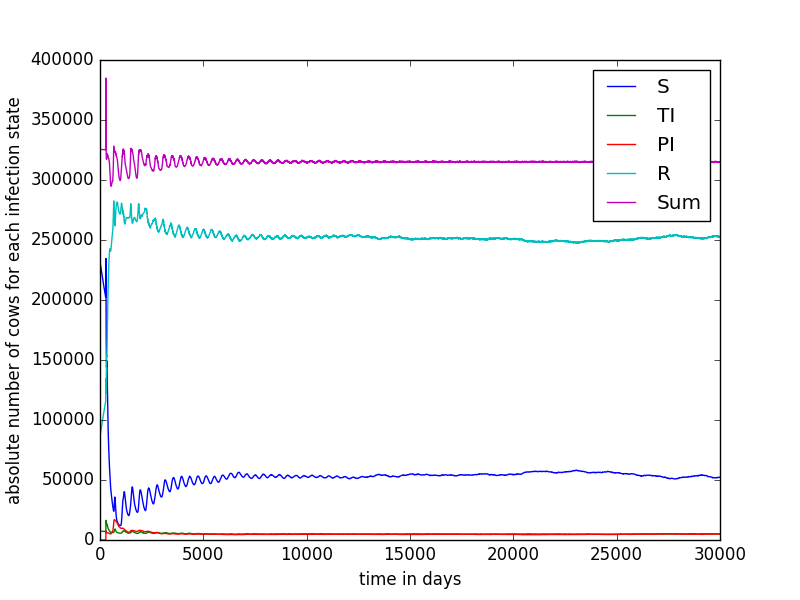
\includegraphics[width=0.95\linewidth,height=\textheight,
keepaspectratio]{cont1totalEndemicNumbers.png} 
\end{minipage}
\begin{minipage}{0.5\textwidth}
\centering
\noindent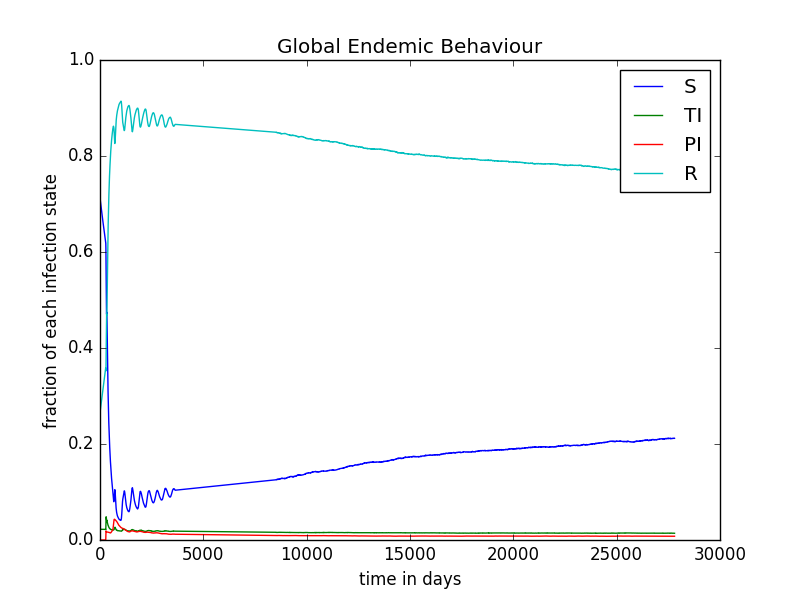
\includegraphics[width=0.95\linewidth,height=\textheight,
keepaspectratio]{cont1endemicFractions.png} 
\end{minipage}
\caption[Endemic Behavior in Containment Strategy One]{Strategy I}
\label{fig:cont1Behav}
\end{figure} 

The difference in the results have to be created by the way the system is initialized. This shows that due to the way of initializing the system far less farms and therefore cows are actually reached by the disease. On the other hand this seems to increase the risk of PIs being produced if an infected animal reaches a farm of purely susceptibles, leading to a slightly higher share of PIs on the total population of the system.

\section{Strategy II - Old BVD Regulation}
As described above the scenario described in this chapter will deal with tests made on every calve a few days after its birth, following the "old" German BVD regulation. A clear drop in the total population of animals, the group of recoverd as well as in the groups of TIs and PIs can be noticed. This drop needs to be due to the testing which is started on day $10000$. Unfortunately the total population does not recover to its full size within the time span of the simulation. The fraction of Rs on the total population drops as far as roughly $55\,\%$, giving rise to the share of susceptibles to about $40\,\%$.
\begin{figure}[htbp]
\begin{minipage}{0.5\textwidth}
\centering
\noindent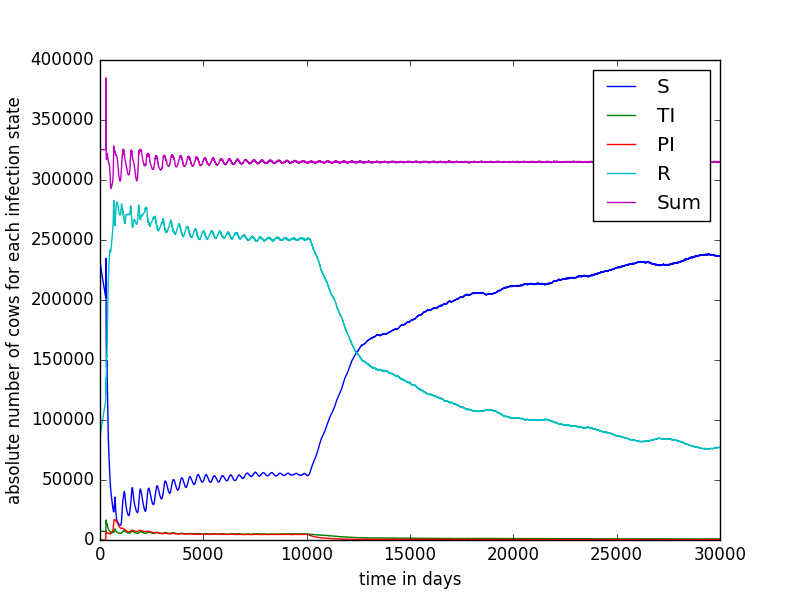
\includegraphics[width=0.95\linewidth,height=\textheight,
keepaspectratio]{cont2totalEndemicNumbers.png} 
\end{minipage}
\begin{minipage}{0.5\textwidth}
\centering
\noindent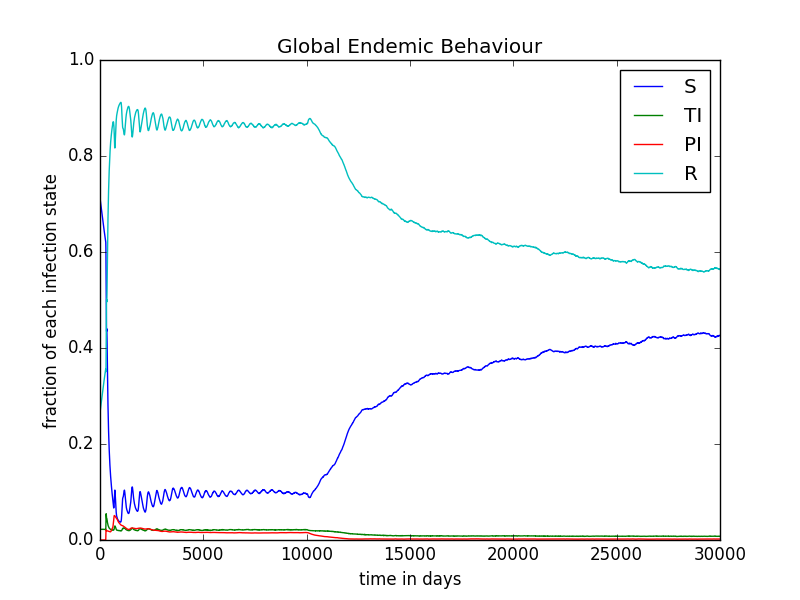
\includegraphics[width=0.95\linewidth,height=\textheight,
keepaspectratio]{cont2endemicFractions.png} 
\end{minipage}
\caption[Endemic Behavior in Containment Strategy Two]{Strategy II}
\label{fig:demographyScen8}
\end{figure}
According to \citep{hofig2014untersuchungen} Switzerland implemented a testing system and prohibited vaccination in 2008, which lowered the PI prevalence from a value between $1.4\,\%-1.8\,\%$ to a value $0.02\,\%-0.06\%$ in the end of 2012. The data acquired in this test looks quite similar. A more precise analysis will be given in the comparison of all strategies in section \ref{chap:stratComparison}. The most important finding of this test is that Testing of all calves alone is not sufficient to fully eradicate the disease as such.

\section{Strategy III - New BVD Regulation}
The new BVD regulation imposes a quarantine after a positive test and shortens the timespan between the first positive test and second test for ensuring the owner of the cow. As discussed in chapter \ref{chap:newBVDRegulationDesc}, this change could be crucial, but due to bonuses paid by most of the federal states, it could also be negligible. 
The most important finding in the figures \ref{fig:contScen3} is that the total population in the system starts to grow exponentially after the start of the tests, which is also why the simulation was stopped after roughly $26000\days$. By the time of writing this thesis it was unclear why this happens. The effects of this rise in population are unclear, but the plot of the shares of the different compartments, especially the subplot of PIs and TIs give the idea that there is no real effect on the prevalence on a global scale. A closer look on farm level might be useful. It can be seen that just as in the Strategy two this Strategy is not sufficient for the eradication of the disease. It even looks as if strategy two was just as efficient as strategy three. A more precise description will be given in \ref{chap:stratComparison}.
This is most likely due to the fact that 
\begin{figure}[htbp]
\begin{minipage}{0.5\textwidth}
\centering
\noindent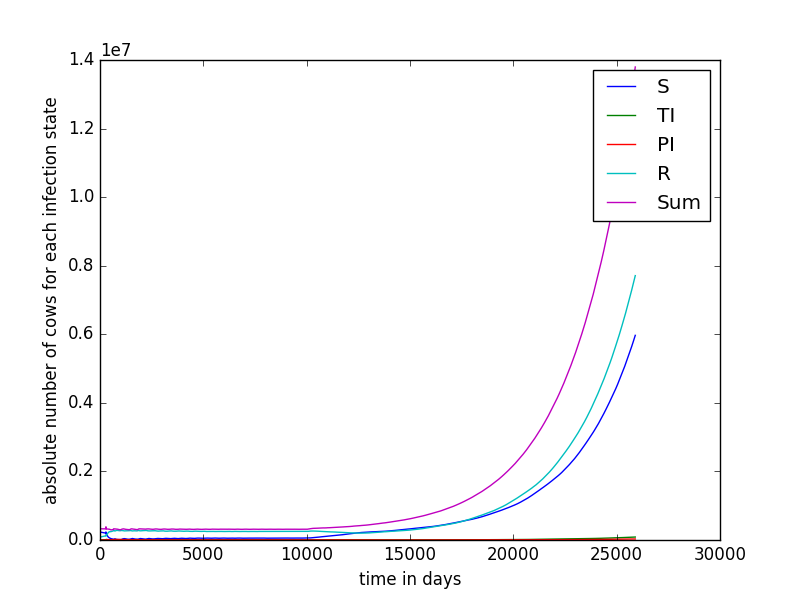
\includegraphics[width=0.95\linewidth,height=\textheight,
keepaspectratio]{cont3totalEndemicNumbers.png} 
\end{minipage}
\begin{minipage}{0.5\textwidth}
\centering
\noindent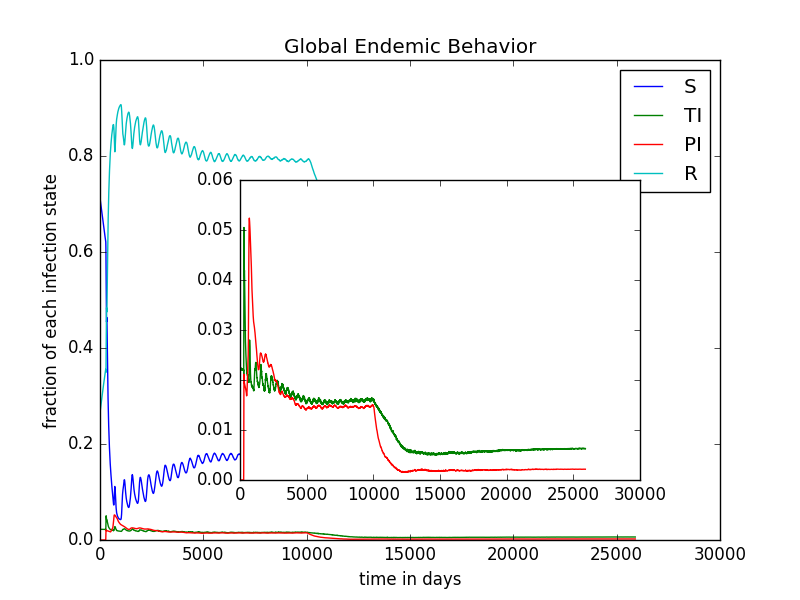
\includegraphics[width=0.95\linewidth,height=\textheight,
keepaspectratio]{cont3endemicFractions.png} 
\end{minipage}
\caption[Endemic Behavior in Containment Strategy Three]{Strategy III}
\label{fig:contScen3}
\end{figure}
As expected this run returns exactly the same results for the first ten thousand days as the simulation for strategies I \& II. 

\section{Strategy IV - New BVD Regulation + Vaccination}
The graphs in figure \ref{fig:contStrat4} expose the same extreme of simulation artifacts as the plots in figure \ref{fig:contScen3}. The total population starts rising exponentialy just after putting the regulation in place. The total number of animals is still relatively stable for the first $5000\days$ of the simulation, growing less then $12\,\%$. Because the simulation time was rising to much, the simulation was aborted after $26000\days$, too. The rise in population in the first $1500\days$ after starting the program is almost only due to more recovered animals and then starts to be split up evenly among the groups of susceptibles and recovereds. In the end the group of immune animals makes up roughly $70\,\%$ of the total population.

\begin{figure}[htbp]
\begin{minipage}{0.5\textwidth}
\centering
\noindent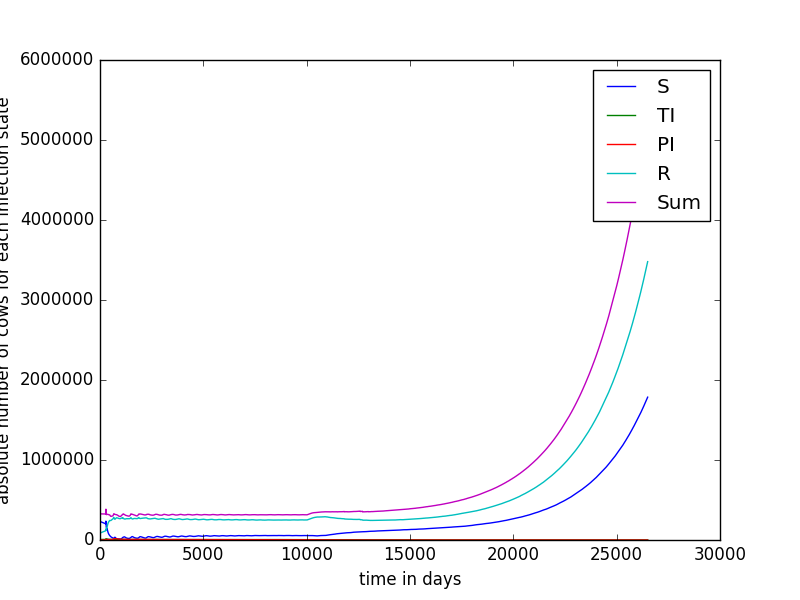
\includegraphics[width=0.95\linewidth,height=\textheight,
keepaspectratio]{cont4totalEndemicNumbers.png} 
\end{minipage}
\begin{minipage}{0.5\textwidth}
\centering
\noindent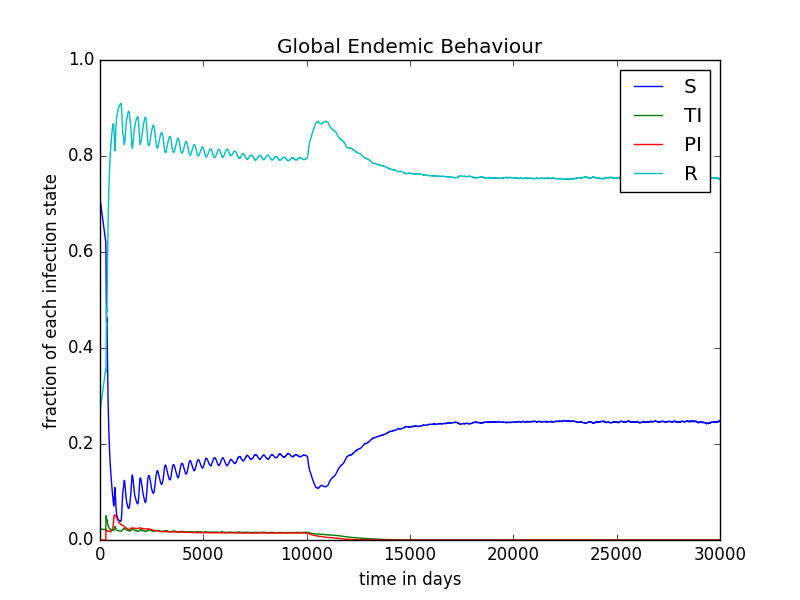
\includegraphics[width=0.95\linewidth,height=\textheight,
keepaspectratio]{cont4endemicFractions.png} 
\end{minipage}
\caption[Endemic Behavior in Containment Strategy Four]{Strategy IV}
\label{fig:contStrat4}
\end{figure}
At the point of writing this thesis the simulation makes no difference between recovered and vaccinated animals, so the rise in recovered animals should actually be due to a big number of animals being vaccinated. Since the rise of animals should be inhibited by the common denominator between the two strategies, it is likely that it is induced by the procedure of the new BVD regulation. The shorter time window for testing an animal again should not be the reason for the problems. The other big change is the quarantine phase in that time frame. There might be an issues with the way the quarantine is implemented, but it could not be found by now and does not (seem to) occur in the following scenarios. If there is a problem with the implementation of the quarantine, it could explain why both strategies need some time to lower the share of PIs on the total population: They need to wait for the PIs to die out instead of accidentally trading them. Of course this only plays a role for the PIs which where tested negative, since the positive tested animals will be removed anyways.
The fact that only $70\,\%$ of the total population are immune at the end of the simulation seems unintuitive at first. The simulation is set up to vaccinate a cow for the first time $42\days$ before its first insemination. The time of first insemination follows a triangle distribution and is located between $480\days$ and $600\days$, making the first vaccination happen between $438\days$ and $558\days$ into the life of the calf. A look at the \ref{fig:demographyScen7} shows that the average lifespan of a cow is in the range of $1500-1800\days$, leaving about a third of the life of an average cow without vaccination and therefore without immunity. This is especially true of the amount of recovered cows is small, because almost no infections take place anymore and therefore the number of calves protected by their maternal antibodies is negligible.


\section{Strategy V - New BVD Regulation + Young Calf Window}
As mentioned in the description of strategies, this strategy will incorporate all rules from the new BVD regulation of Germany as well as an added herd-level detection mechanism, the Young Calf Window. As discussed in the description of the Young Calf Window, the scenarios V \& VI will be split up into two scenarios each. One of which will test the YCW once every half a year (a) whereas the other subscenario (b) tests cows for the YCW only once a year.

\subsection{Strategy Va}

\begin{figure}[htbp]
\begin{minipage}{0.5\textwidth}
\centering
\noindent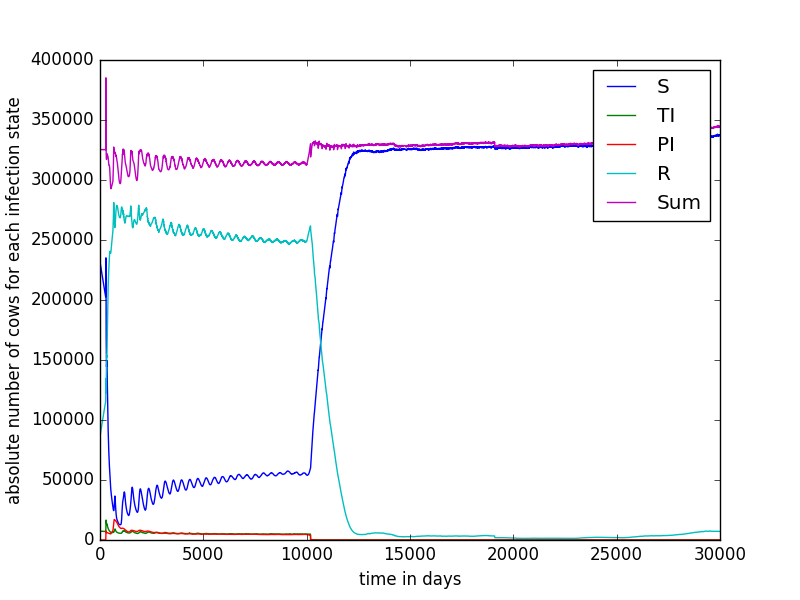
\includegraphics[width=0.95\linewidth,height=\textheight,
keepaspectratio]{cont5totalEndemicNumbers.png} 
\end{minipage}
\begin{minipage}{0.5\textwidth}
\centering
\noindent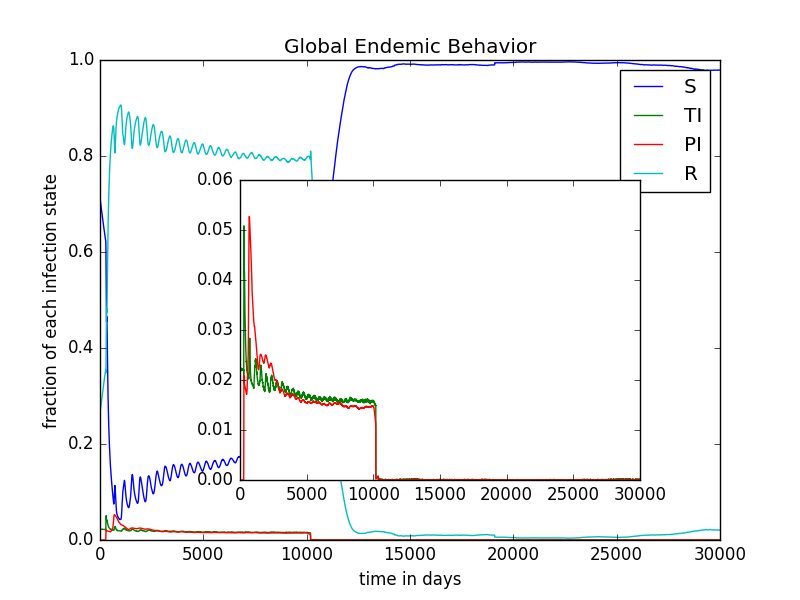
\includegraphics[width=0.95\linewidth,height=\textheight,
keepaspectratio]{cont5pendemicFractions.png} 
\end{minipage}
\caption[Endemic Behavior in Containment Strategy Five A]{Strategy Va}
\label{fig:contStrat5a}
\end{figure}
The plots of the results of the simulation for strategy Va shown in figure \ref{fig:contStrat5a} are the first plots showing a relaxation of the total population size to its initial value. This is only possible after the disease as such has almost completely been eradicated. The time needed for the eradication process is exactly the time set for the Jungtierfenster to take place. In other words exactly half a year after the program has been started, the share of PIs and TIs drops to almost zero. 
Since the program includes no vaccination, all recovered animals in the simulation need to have had contact with infected animals before. This means that there are still infected animals in the system. They might just be put into the system by the cow well farm. Another test is supposed to find out how big of a percentage of PIs can be brought into the system by the cow well farm. 
The explanation for the drop in the population shares of TIs and PIs is quite straight forward: When the YCW is carried out for the first time, all farms are scanned. The prevalence of recovered animals in a herd that recently used to be home to a PI is around $90\,\%$, which makes it almost impossible to not detect any of them. After one of them has been detected, the whole farm will be scanned. With a $99.8\,\%$ probability infecteds will be discovered. Roughly $75\,\%$ of them will be removed directly, the other $25\,\%$ will be removed or die within $40\days$. Another test was performed to find out if the infected animals staying in the system where introduced by the cow well farm by setting the number of PIs in the cow well farm to zero. Still a nonzero amount of TIs and PIs was observed.
\subsection{Strategy Vb}
The results from strategy Vb (figure \ref{fig:contStrat5b}) look almost exactly the same as the results from strategy Va. Two major differences between the two scenarios is that the drop in PIs and TIs takes place half a year later, a year after installing the program and that the program seems to be even more effective in eradicating the disease. Still the system exposes fluctuations in the numbers of recovereds and susceptibles around $21000\days$, indirectly indicating the presence of TIs and/or PIs. The peak in the total population after the start of the program is a little bit more pronounced in comparison to strategy Va.
\begin{figure}[htbp]
\begin{minipage}{0.5\textwidth}
\centering
\noindent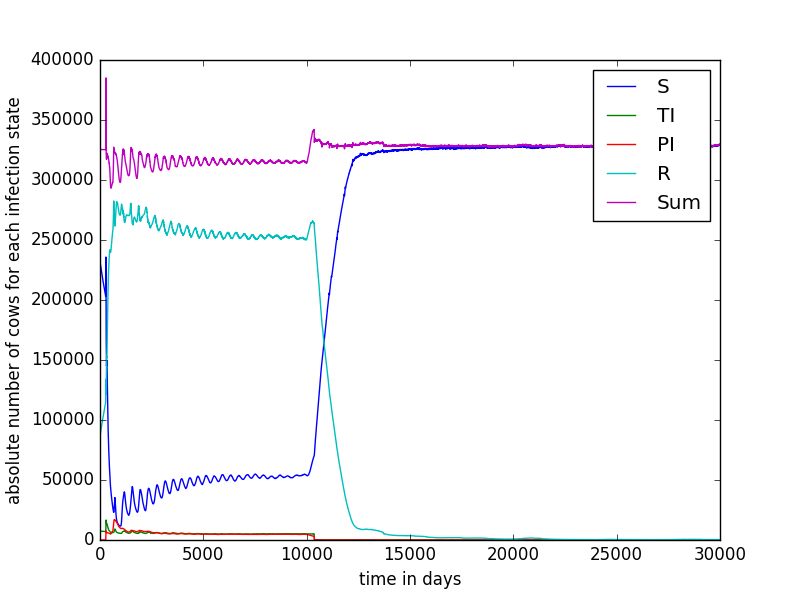
\includegraphics[width=0.95\linewidth,height=\textheight,
keepaspectratio]{cont5btotalEndemicNumbers.png} 
\end{minipage}
\begin{minipage}{0.5\textwidth}
\centering
\noindent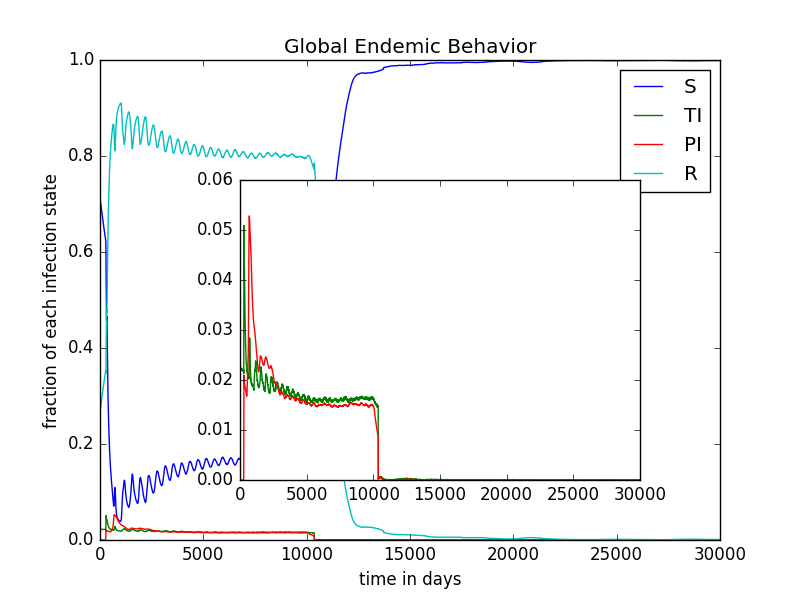
\includegraphics[width=0.95\linewidth,height=\textheight,
keepaspectratio]{cont5bpendemicFractions.png} 
\end{minipage}
\caption[Endemic Behavior in Containment Strategy Five B]{Strategy Vb}
\label{fig:contStrat5b}
\end{figure}

\section{Strategy VI - New BVD Regulation + Vaccination + Young Calf Window} 
The final composition of methods of containment incorporates the testing of calves following the most recent BVD regulation, vaccination and the YCW. The section for this strategy is split up into two sections for the different configurations of the jungtierfenster.
\subsection{Strategy VIa}

\begin{figure}[htbp]
\begin{minipage}{0.5\textwidth}
\centering
\noindent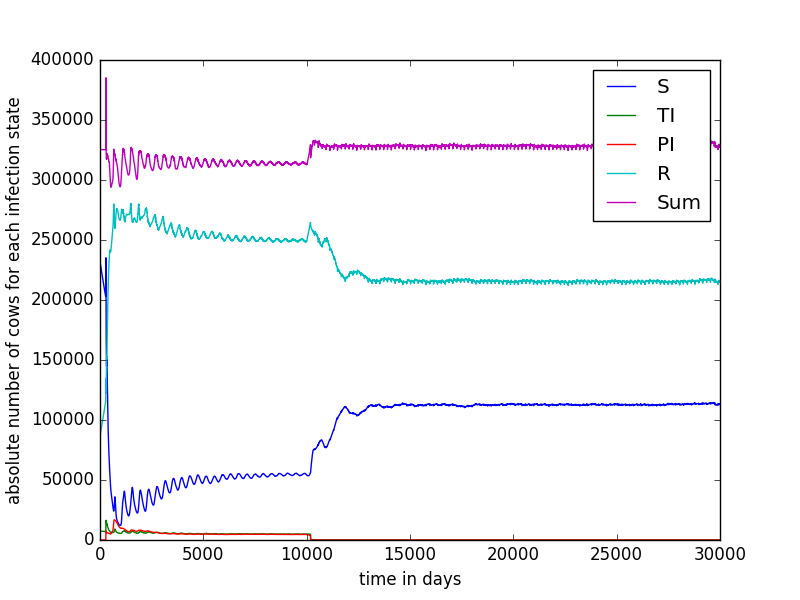
\includegraphics[width=0.95\linewidth,height=\textheight,
keepaspectratio]{cont6totalEndemicNumbers.png} 
\end{minipage}
\begin{minipage}{0.5\textwidth}
\centering
\noindent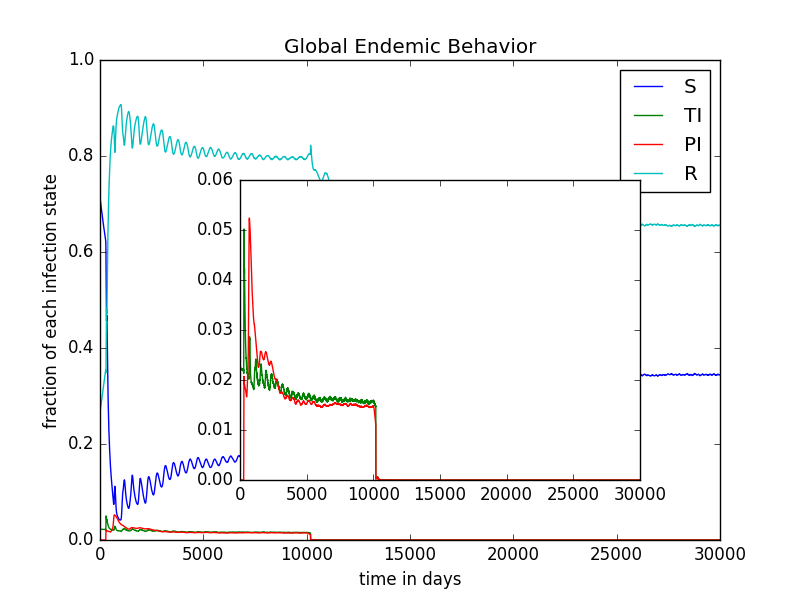
\includegraphics[width=0.95\linewidth,height=\textheight,
keepaspectratio]{cont6pendemicFractions.png} 
\end{minipage}
\caption[Endemic Behavior in Containment Strategy Six A]{Strategy VIa}
\label{fig:contStrat6a}
\end{figure}
The very imprecise depiction of the results of the simulation for strategy VIa in figure \ref{fig:contStrat6a} resemble the ones from strategy Va quite well including the shape of the peaks in total population size as well as the number of recovered animals right after the first screening of the YCW. The major difference is that due to the vaccination the number of recovered animals stays at roughly $70\,\%$. This can easily be explained by the failed missing distinction between recovered and vaccinated animals as it is described for strategy IV. The share of immune animals tends to the same value of roughly $70\,\%$ as for scenario IV. 
\subsection{Strategy VIb}
The last of all tested strategies exposes no new characteristics. The plots in figure \ref{fig:contStrat6b} show the same behavior as the ones above with the only difference being a higher peak in the total number of cows and in the number of recovered animals. 
\begin{figure}[htbp]
\begin{minipage}{0.5\textwidth}
\centering
\noindent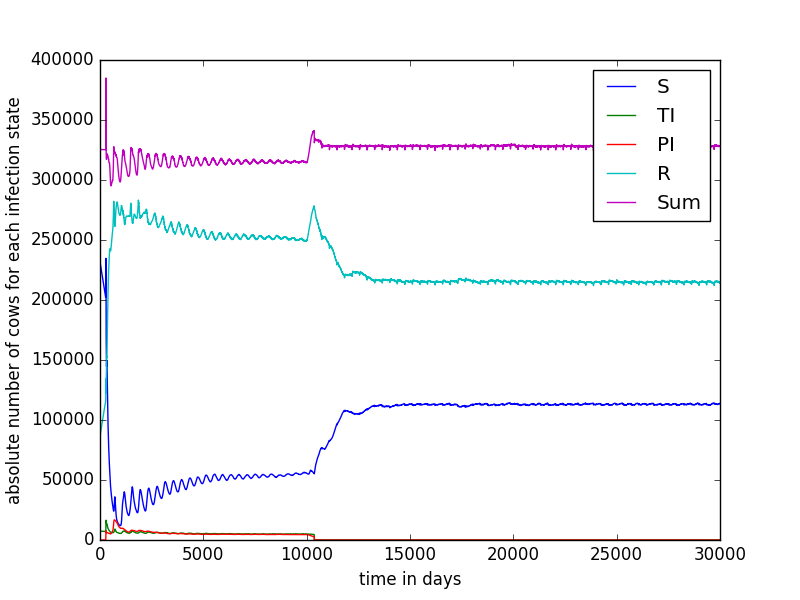
\includegraphics[width=0.95\linewidth,height=\textheight,
keepaspectratio]{cont6btotalEndemicNumbers.png} 
\end{minipage}
\begin{minipage}{0.5\textwidth}
\centering
\noindent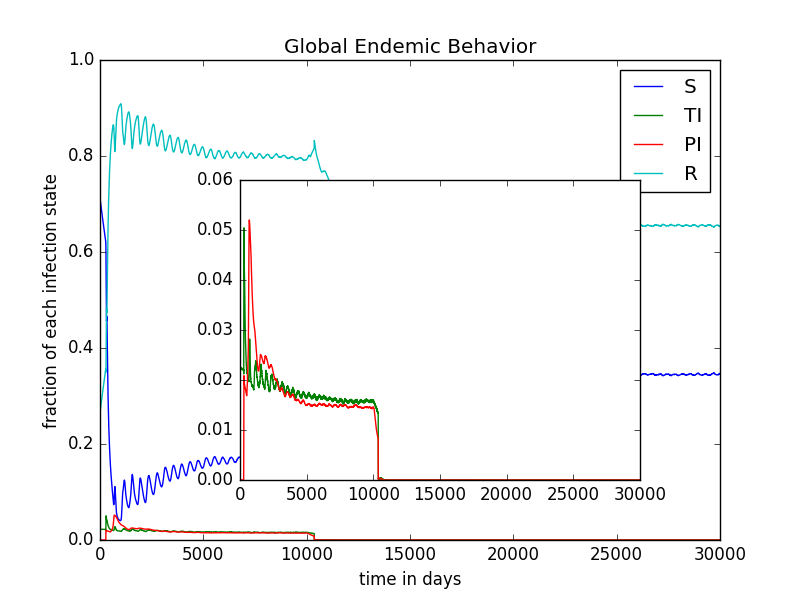
\includegraphics[width=0.95\linewidth,height=\textheight,
keepaspectratio]{cont6bpendemicFractions.png} 
\end{minipage}
\caption[Endemic Behavior in Containment Strategy Six B]{Strategy VIb}
\label{fig:contStrat6b}
\end{figure}

\section{Comparison of the different Strategies}\label{chap:stratComparison}
Figure \ref{fig:contComp1} shows the prevalences of PIs and TIs of the first four scenarios. The two test scenarios in strategy II and III are almost identical with strategy III even being slightly less effective than strategy II. This could be caused by the peculiar rise of the population. The PI prevalence is lowered to $0.2\,\%$ after roughly $5.5\,\text{years}$. This means that $87.5\,\%$ of all PIs have been removed from the system. According to \citep{personalCom} the PI prevalence in Thuringia has been lowered from $0.44\,\%$ in 2011 to $0.05\,\%$ 2015, which would be roughly the same percentage ($88.6\,\%$) of all PIs removed in 4 years. This means that the testing in the simulation removes roughly the same percentage of PIs in approximately 1.4 times the time that the testing takes in reality. Expanding the plot beyond the time of $18000\days$ reveals that the prevalence of PIs and TIs keeps declining in scenario 2, and continuous rising in scenario 3.T
\begin{figure}[htbp]
\centering
\noindent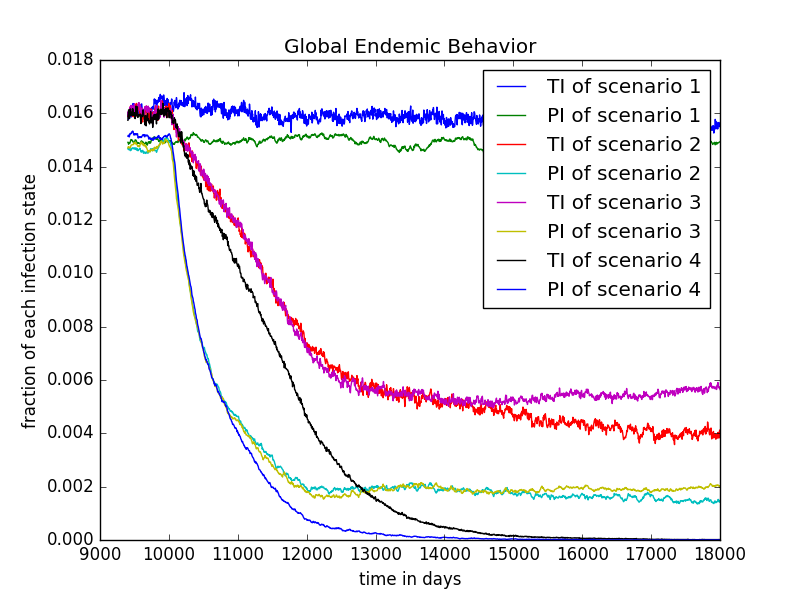
\includegraphics[width=0.8\linewidth,height=\textheight,
keepaspectratio]{comp1b4endemicFractions.png} 
\caption[Comparison of Prevalences for the Strategies I-IV]{}
\label{fig:contComp1}
\end{figure}
\begin{figure}[htbp]
\centering
\noindent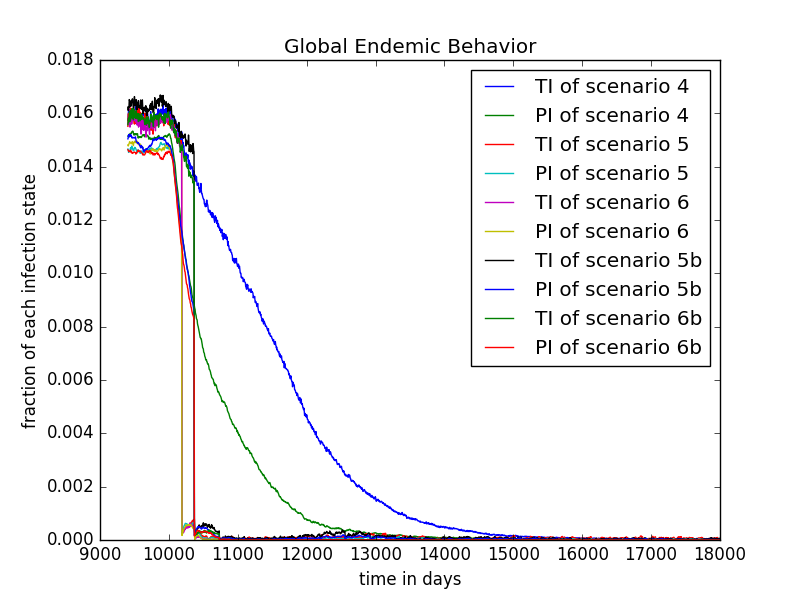
\includegraphics[width=0.8\linewidth,height=\textheight,
keepaspectratio]{comp4t6bendemicFractions.png} 
\caption[Comparison of Prevalences for the Strategies IV-VIb]{}
\label{fig:contComp2}
\end{figure}